\documentclass[a4paper]{article}
\usepackage{xcolor}
\usepackage{listings}
\usepackage{tikz}
\usepackage{pifont}
\usepackage{amsmath}
\usepackage{multirow}
\usepackage{url}
% Optional but recommended: geometry package gives you slightly wider margins 
% which is great for algorithmic reports
% Geometry is configured later with explicit top/bottom/left/right values.

% Define custom colors
\definecolor{codegreen}{RGB}{34,139,34}
\definecolor{codegray}{RGB}{110,118,129}
\definecolor{codepurple}{RGB}{163,73,164}
\definecolor{backcolour}{RGB}{247,248,250}
\definecolor{codeblue}{RGB}{0,92,197}
\definecolor{codeorange}{RGB}{191,97,15}
\definecolor{codeteal}{RGB}{0,128,128}
\definecolor{codered}{RGB}{196,43,28}

% Global setup for listings
\lstset{
    language=Python,
    basicstyle=\ttfamily\small,
    keywordstyle=\color{codeblue}\bfseries,
    keywordstyle=[2]\color{codered}\bfseries,
    commentstyle=\color{codegreen}\itshape,
    stringstyle=\color{codepurple},
    numberstyle=\scriptsize\color{codegray},
    identifierstyle=\color{black},
    emph={add_bulb,remove_bulb,has_bulb,can_place_bulb,is_goal_state,compute_illumination,count_adjacent_bulbs,number_constraint_violations},
    emphstyle=\color{codeorange}\bfseries,
    morekeywords=[2]{self,True,False,None},
    numbers=left,
    numbersep=10pt,
    stepnumber=1,
    backgroundcolor=\color{backcolour},
    frame=single,
    framerule=0.5pt,
    rulecolor=\color{codegray},
    xleftmargin=12pt,
    framexleftmargin=10pt,
    framesep=6pt,
    breaklines=true,
    breakatwhitespace=false,
    showstringspaces=false,
    showspaces=false,
    showtabs=false,
    keepspaces=true,
    tabsize=4,
    captionpos=b,
    upquote=true
}
\usepackage[utf8]{inputenc}
\usepackage[T1]{fontenc}
\usepackage{CJKutf8}
\usepackage[english,vietnamese]{babel}
\usepackage{tocloft}
\usepackage{a4wide,amssymb,epsfig,latexsym,multicol,array,hhline,fancyhdr}
\usepackage{lastpage}
\usepackage[lined,boxed,commentsnumbered]{algorithm2e}
\usepackage{xcolor}
\usepackage{graphicx}
\usepackage{array}
\usepackage{tabularx, caption}
\usepackage{multirow}
\usepackage{multicol}
\usepackage{rotating}
\usepackage{placeins}
\usepackage[
    a4paper,
    left=2cm,
    right=2cm,
    top=2.5cm,
    bottom=2.5cm,
    includeheadfoot,
    headsep=0.8cm,
    footskip=0.8cm
]{geometry}
\usepackage{setspace}
\usepackage{eso-pic}
\usepackage{tikz}
\usepackage{xfrac}
\usepackage{bm}

\usepackage{biblatex}
\addbibresource{references.bib}

\usepackage[colorlinks]{hyperref}
\usepackage{mdframed}
\captionsetup[table]{name=Table}
\captionsetup[figure]{name=Figure}
\hypersetup{urlcolor=blue,linkcolor=black,citecolor=black,colorlinks=true}
\usetikzlibrary{arrows,backgrounds}
\definecolor{mathblue}{RGB}{0,114,188}
\newtheorem{theorem}{{\bf Theorem}}
\newtheorem{property}{{\bf Property}}
\newtheorem{proposition}{{\bf Proposition}}
\newtheorem{corollary}[proposition]{{\bf Corollary}}
\newtheorem{lemma}[proposition]{{\bf Lemma}}
\AtBeginDocument{\renewcommand{\listfigurename}{List of Figures}}
\AtBeginDocument{\renewcommand{\listtablename}{List of Tables}}
\AtBeginDocument{\renewcommand*\contentsname{Contents}}
\AtBeginDocument{\renewcommand*\refname{References}}
\AtBeginDocument{\renewcommand{\partname}{Part}}
\setlength{\headheight}{40pt}

\pagestyle{fancy}
\fancyhead{}
\fancyhead[L]{
 \begin{tabular}{rl}
    \begin{picture}(25pt,15pt)
        \put(0,-8pt){
\includegraphics[width=20pt]{bia/logo.png}}
      \end{picture}
    &
\hspace*{-0.9cm}\begin{tabular}{l}
\textbf{\ttfamily Ho Chi Minh City University of Technology (HCMUT)}\\
\textbf{\ttfamily Faculty of Computer Science and Engineering}
\end{tabular}
 \end{tabular}
}
\fancyfoot{}
\fancyfoot[L]{\scriptsize \ttfamily \hyperref[tocpage]{CC01 - Group 36}}
\fancyfoot[R]{\scriptsize \ttfamily Page {\thepage}/\pageref{LastPage}}

\renewcommand{\headrulewidth}{0.3pt}
\renewcommand{\footrulewidth}{0.3pt}
\setlength{\parindent}{0pt}
\setlength{\parskip}{3pt}

\usepackage{float}
\usepackage{caption}
\usepackage{calc}
\usepackage[table]{xcolor}
\usepackage{booktabs}
\usepackage{longtable}
\setlength{\tabcolsep}{8pt} % Giảm khoảng cách cột để bảng dễ vừa trang hơn
\renewcommand{\arraystretch}{1.5}

\usepackage{titlesec}
\renewcommand{\partname}{Part}
\titleformat{\part}[display]
    {\normalfont\huge\bfseries\centering}
    {\partname~\thepart}
    {20pt}
    {\Huge}
\titlespacing*{\part}{0pt}{0pt}{40pt}
\usepackage{tcolorbox}
\usepackage{amsmath}
\DeclareMathOperator{\arccot}{arccot}
\usepackage{url}

\usepackage{listings}
\usepackage{pdflscape}

\newcommand{\zh}[1]{{\begin{CJK*}{UTF8}{bsmi}#1\end{CJK*}}}

\captionsetup[table]{skip=2pt}

\begin{document}

% TITLE PAGE
\begin{titlepage}
\AddToShipoutPicture*{%
  \put(0,0){%
    
\includegraphics[width=\paperwidth,height=\paperheight]{bia/bia.pdf}
  }%
}
\vspace*{-1cm}
\begin{center}
VIETNAM NATIONAL UNIVERSITY, HO CHI MINH CITY \\[1mm]
UNIVERSITY OF TECHNOLOGY \\[1mm]
FACULTY OF COMPUTER SCIENCE AND ENGINEERING
\end{center}

\vspace{1cm}

\begin{figure}[h!]
\begin{center}

\includegraphics[width=3cm]{bia/logo.png}
\end{center}
\end{figure}

\vspace{0cm}


\begin{center}

\begin{tabular}{c}
\multicolumn{1}{c}{\textbf{{\Large Deep Learning and Its Applications (CO3133)}}}\\
~~\\
\hline
\\
\multicolumn{1}{c}{\textbf{{\Large Assignment 1}}}\\
\\
\textbf{\textit{{\Large
Foundations of Deep Learning Pipelines and Architectures}}}\\
\\
\textbf{\textit{{
 Topic: From Linear Models to Modern Sequence Models:
   }}}
\\
\textbf{\textit{{
   A Comparative Study for Image Classification.}}}\\
\\
\hline
\end{tabular}
\end{center}

\vspace{1cm}
\begin{table}[h]
\centering
\begin{tabular}{p{6cm} r}

\multicolumn{2}{l}{\textbf{Instructor}: Lê Thành Sách} \\
\multicolumn{2}{l}{\textbf{Class}: CC01} \\
\multicolumn{2}{l}{\textbf{Semester}: 1 -- Year 2026--2027} \\
\\[6pt]

\textbf{Students:} &  \\

Trịnh Lê Minh      & 2352765 \\
Trần Phước Sang    & 2353044 \\
Đặng Trần Thái Bảo & 2452120  \\

% \textbf{Group: 36} 
\end{tabular}
\end{table}


\vspace{1cm}
\begin{center}
{\footnotesize HO CHI MINH CITY, SEPTEMBER 2026}
\end{center}
\end{titlepage}
\pagebreak

\vspace{1em}

\clearpage

\label{tocpage}
\tableofcontents
\listoffigures
\listoftables

\newpage
\section*{Workload Distribution}
\addcontentsline{toc}{section}{Workload Distribution}

\begin{table}[H]
\centering
\renewcommand{\arraystretch}{1.3}
\begin{tabular}{|c|l|c|c|c|}
\hline
\textbf{No} & \textbf{Name} & \textbf{Student's ID} & \textbf{Work} & \textbf{Contribution} \\
\hline
1 & Trịnh Lê Minh   & 2352765 & Main Develop & 100\% \\
\hline
2 & Trần Phước Sang & 2353044 & Verify Dev and Outline Report & 100\% \\
\hline
3 & Đặng Trần Thái Bảo     & 2452120  & Complete Report and Slides & 100\% \\
\hline
\end{tabular}
\caption{Workload allocation among team members.}
\label{tab:workload_distribution}
\end{table}


\clearpage

\part{Problem and Data Description}
\section{Problem Formulation}

\textbf{Motivation.} Fashion-MNIST is a standard image-classification benchmark for evaluating machine-learning pipelines on grayscale clothing images. The task provides a controlled setting for comparing a linear classifier with a multilayer perceptron while preserving challenges such as visually similar clothing categories.

\textbf{Input.} Each input is a grayscale image with shape $1\times28\times28$. Pixel intensities are represented as floating-point values in $[0,1]$ before normalization and are flattened to 784 features by both models.

\textbf{Output.} The target is one of ten Fashion-MNIST classes. Each prediction corresponds to one image and is obtained from the class with the largest output logit.

\textbf{Mathematical formulation.}
\begin{equation}
    \hat{y} = f_{\theta}(x),
    \qquad
    \theta^{*} = \arg\min_{\theta}\frac{1}{N}\sum_{i=1}^{N}
    \mathcal{L}\bigl(f_{\theta}(x_i), y_i\bigr).
    \label{eq:problem-formulation}
\end{equation}
For a batch of images, the models minimize the cross-entropy loss over the ten-class target distribution.

\textbf{Main difficulties.} The main challenges are distinguishing visually similar classes such as Shirt, T-shirt/top, Pullover, and Coat; handling the high-dimensional flattened input; and controlling overfitting while using a fully connected architecture.

\section{Dataset Description}

\begin{table}[H]
    \centering
    \caption{Dataset summary.}
    \label{tab:dataset-summary}
    \begin{tabularx}{\textwidth}{@{}lX@{}}
        \toprule
        Property & Description \\
        \midrule
        Source and version & TODO \\
        License & TODO \\
        Collection and labeling & TODO \\
        Number of samples & TODO \\
        Annotation format & TODO \\
        Storage size and formats & TODO \\
        Biases and limitations & TODO \\
        \bottomrule
    \end{tabularx}
\end{table}

\begin{table}[H]
    \centering
    \caption{Class or target distribution.}
    \label{tab:target-distribution}
    \begin{tabular}{@{}lrr@{}}
        \toprule
        Class / target & Count & Percentage \\
        \midrule
        Class A & TODO & TODO \\
        Class B & TODO & TODO \\
        Total & TODO & 100\% \\
        \bottomrule
    \end{tabular}
\end{table}

\section{Exploratory Data Analysis}

\subsection{Core EDA}

The core EDA describes the dataset size, tensor shape, pixel range, pixel statistics, class distribution, and representative images. All random examples are selected reproducibly using seed 42.

\begin{figure}[H]
    \centering
    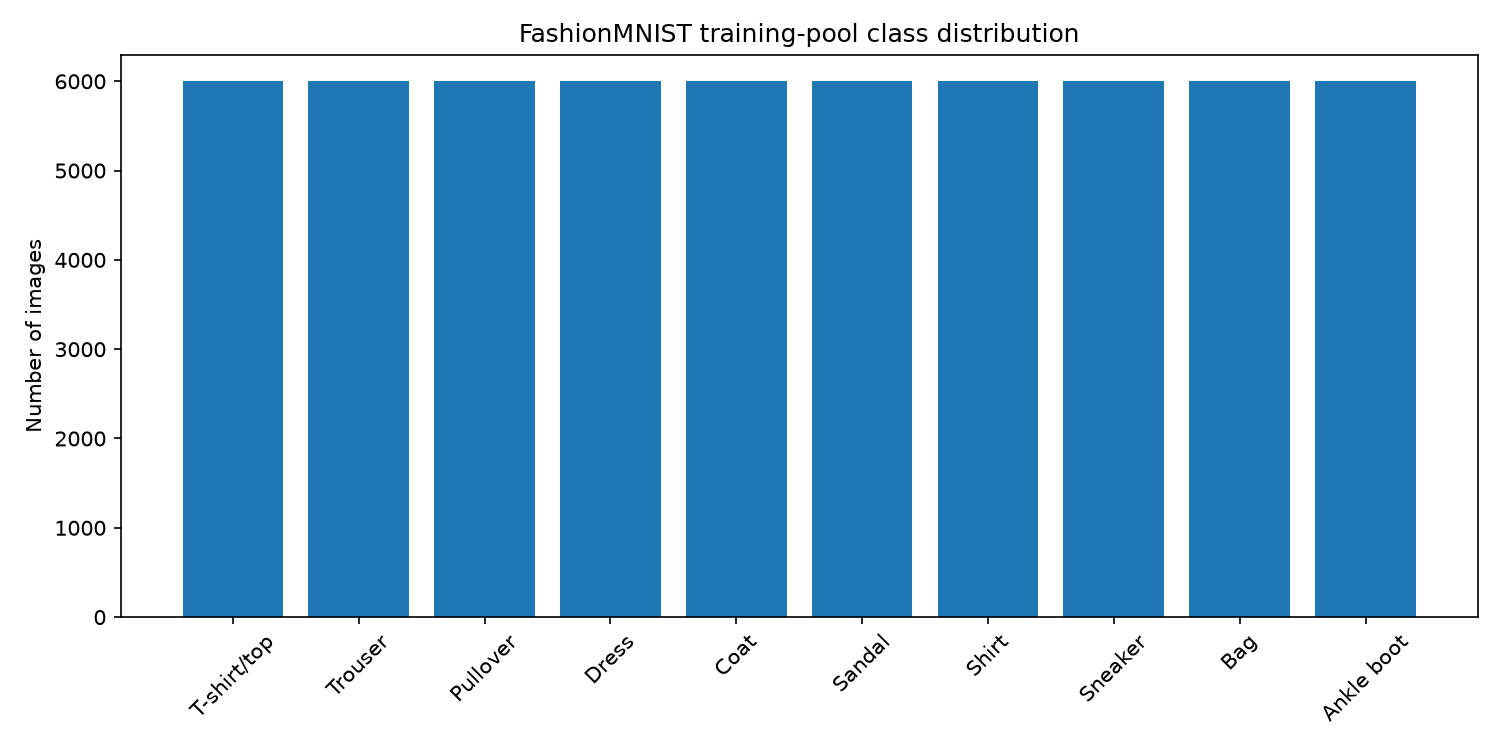
\includegraphics[width=0.9\textwidth]{../../Assignment1/outputs/eda/class_distribution.png}
    \caption{Fashion-MNIST training-pool class distribution.}
    \label{fig:eda-class-distribution}
\end{figure}

The class distribution is perfectly balanced, with 6,000 images for each of the ten classes in the official training pool. This balance reduces the risk that the classifiers are dominated by a majority class.

\begin{figure}[H]
    \centering
    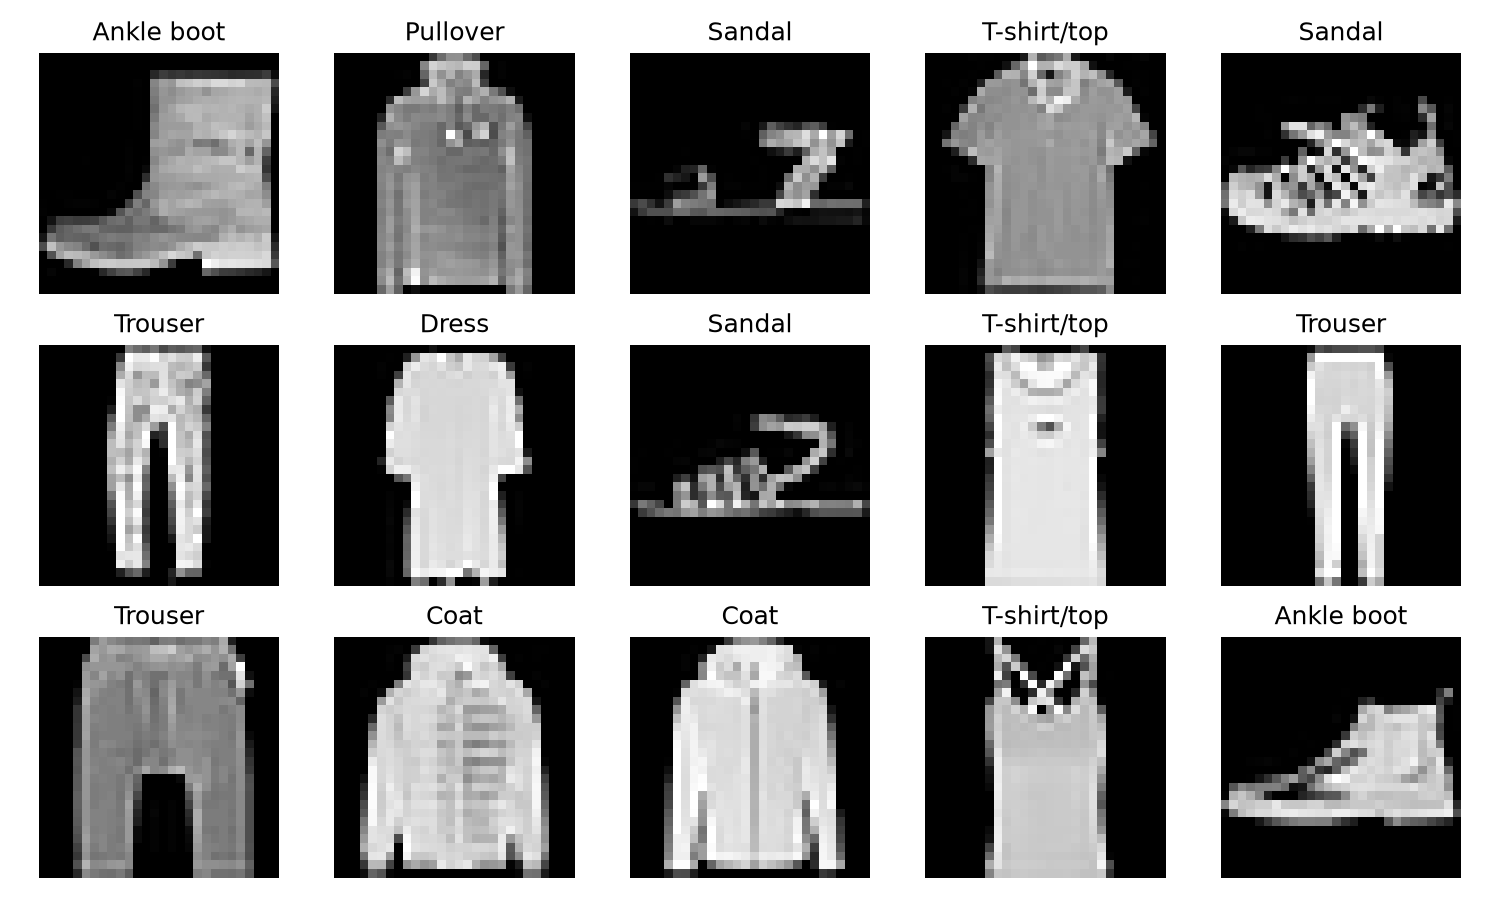
\includegraphics[width=0.9\textwidth]{../../Assignment1/outputs/eda/random_examples.png}
    \caption{Reproducibly selected Fashion-MNIST training examples.}
    \label{fig:eda-random-examples}
\end{figure}

The sampled images confirm that the dataset contains centered grayscale clothing objects with visually meaningful class labels. They also illustrate within-class variation in pose, shape, and intensity, which motivates using both a linear baseline and a nonlinear MLP model.

\begin{table}[H]
    \centering
    \caption{EDA statistics.}
    \label{tab:eda-statistics}
    \begin{tabular}{@{}lrr@{}}
        \toprule
        Statistic & Value & Notes \\
        \midrule
        Mean & 0.2860 & Computed on training-pool pixels scaled to $[0,1]$. \\
        Standard deviation & 0.3530 & Computed on training-pool pixels scaled to $[0,1]$. \\
        Minimum / maximum & 0.0 / 1.0 & Raw pixel values after scaling. \\
        Missing or invalid values & 0 detected & No missing-value handling was required. \\
        \bottomrule
    \end{tabular}
\end{table}

The images are represented as $1\times28\times28$ tensors with pixel values in $[0,1]$. The mean and standard deviation provide the normalization values used by the data-loading pipeline.

\subsection{Task-Specific EDA (Classification)}

For the classification task, the EDA additionally examines the geometry of the image representations and the similarity between class-level average images.

\begin{figure}[H]
    \centering
    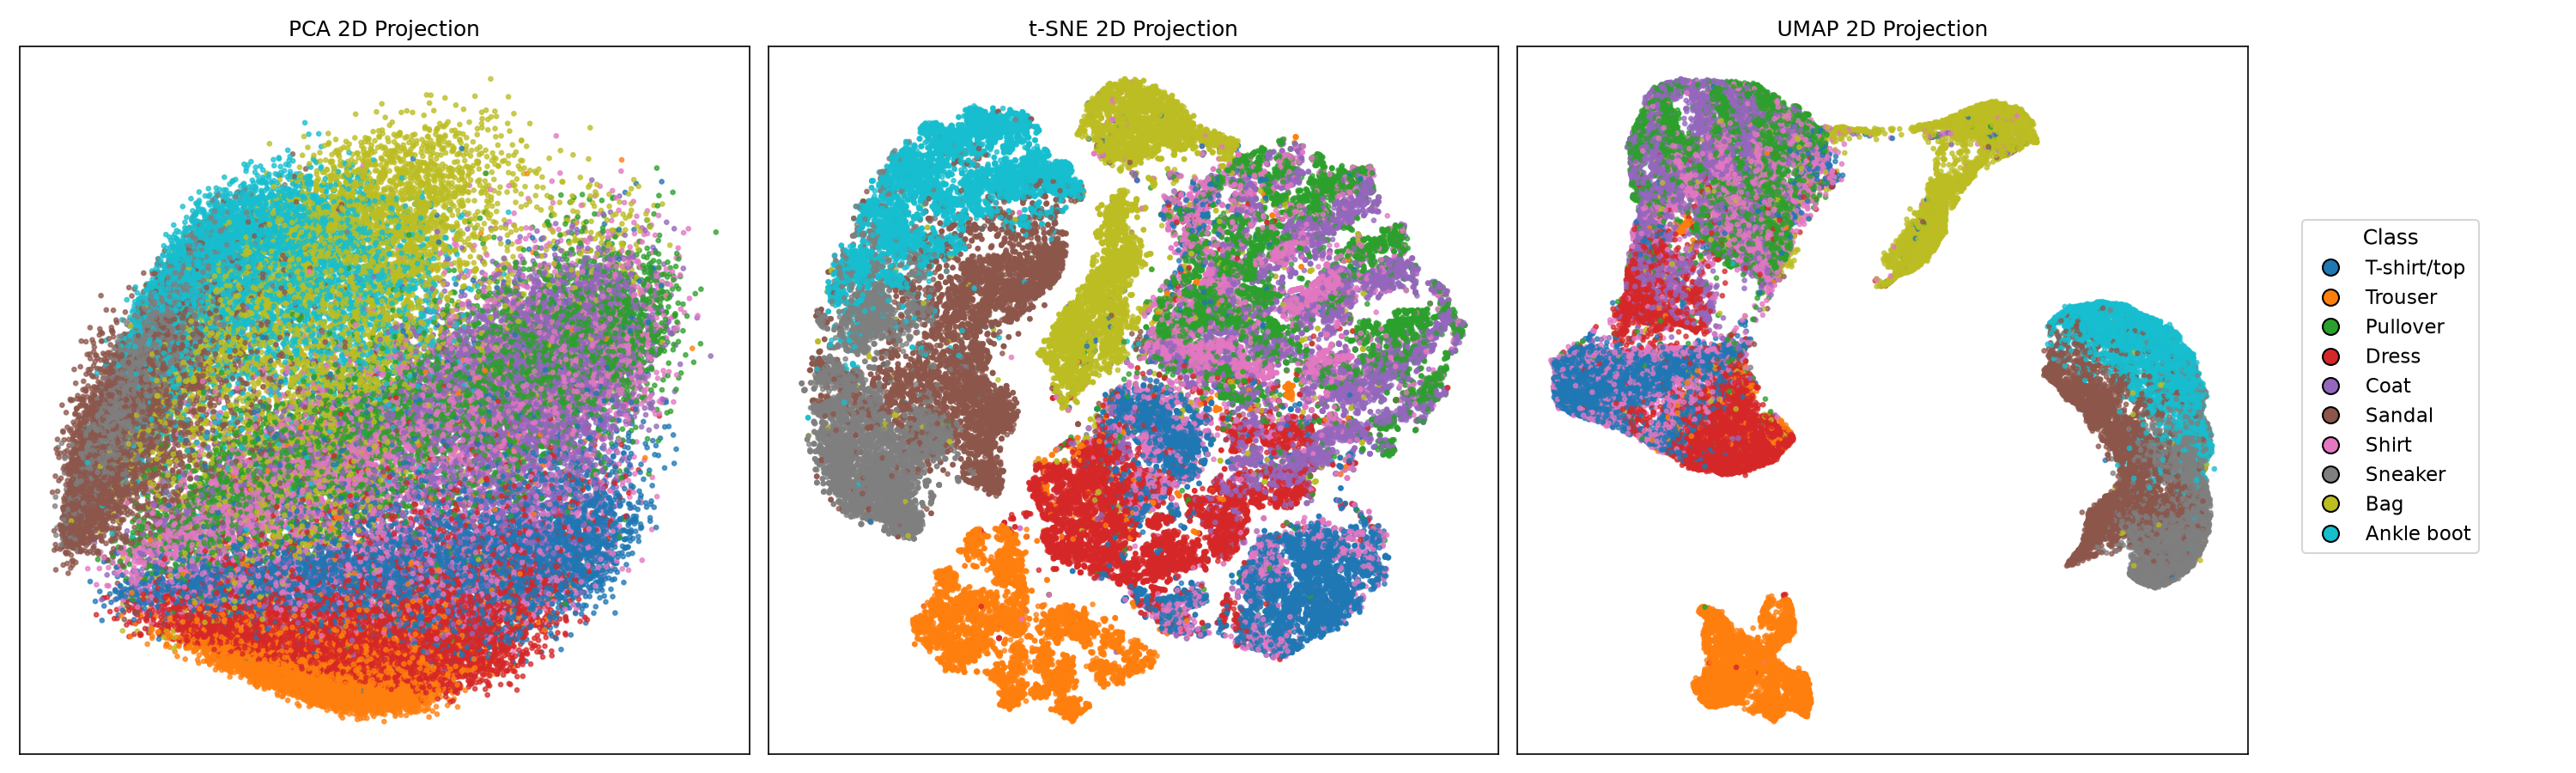
\includegraphics[width=\textwidth]{../../Assignment1/outputs/eda/dimensionality_reduction.png}
    \caption{PCA, t-SNE, and UMAP projections of sampled Fashion-MNIST images.}
    \label{fig:eda-dimensionality-reduction}
\end{figure}

The dimensionality-reduction views show that some classes form relatively coherent groups, while visually similar clothing categories overlap. PCA provides a broad linear view, whereas t-SNE and UMAP reveal more localized nonlinear structure. These projections suggest that footwear classes are often easier to separate, while upper-body categories may require more expressive decision boundaries.

\begin{figure}[H]
    \centering
    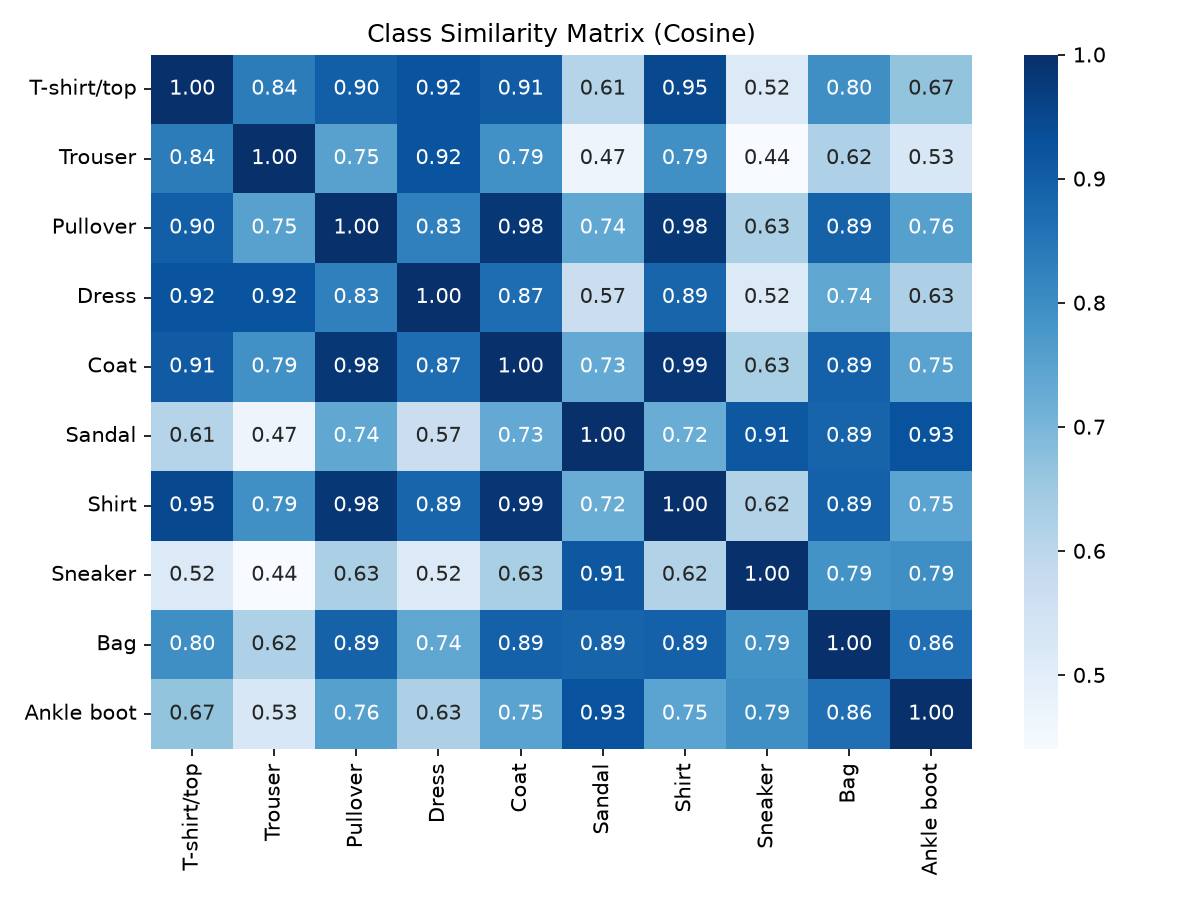
\includegraphics[width=0.78\textwidth]{../../Assignment1/outputs/eda/class_similarity_matrix.png}
    \caption{Cosine similarity between class-level mean images.}
    \label{fig:eda-class-similarity}
\end{figure}

The cosine-similarity matrix highlights pairs of classes with similar average visual structure. For example, Pullover--Coat and Coat--Shirt have high similarity, while Sandal--Trouser and Sneaker--Trouser are less similar. The high similarity among several upper-body classes indicates likely confusion regions for classification and motivates the later error analysis.

\section{Data Splitting}

Describe the train, validation, and test partitions. State whether the split is official or custom, the random seed, stratification strategy, split unit, leakage prevention, and any subset selection rules.

\begin{table}[H]
    \centering
    \caption{Data split configuration.}
    \label{tab:data-split}
    \begin{tabular}{@{}lrrl@{}}
        \toprule
        Split & Samples & Percentage & Selection rule \\
        \midrule
        Train & TODO & TODO & TODO \\
        Validation & TODO & TODO & TODO \\
        Test & TODO & TODO & TODO \\
        \bottomrule
    \end{tabular}
\end{table}

\section{Preprocessing}

Describe cleaning, resizing, normalization, tokenization, padding, augmentation, invalid annotation handling, and the input tensor shape(s).

\begin{table}[H]
    \centering
    \caption{Preprocessing pipeline.}
    \label{tab:preprocessing}
    \begin{tabularx}{\textwidth}{@{}lXX@{}}
        \toprule
        Stage & Operation & Configuration \\
        \midrule
        Cleaning & TODO & TODO \\
        Transformation & TODO & TODO \\
        Normalization & TODO & TODO \\
        Augmentation & TODO & TODO \\
        Tensor shape & TODO & TODO \\
        \bottomrule
    \end{tabularx}
\end{table}

\begin{figure}[H]
    \centering
    % Suggested image filename: graphics/preprocessed-batch.png
    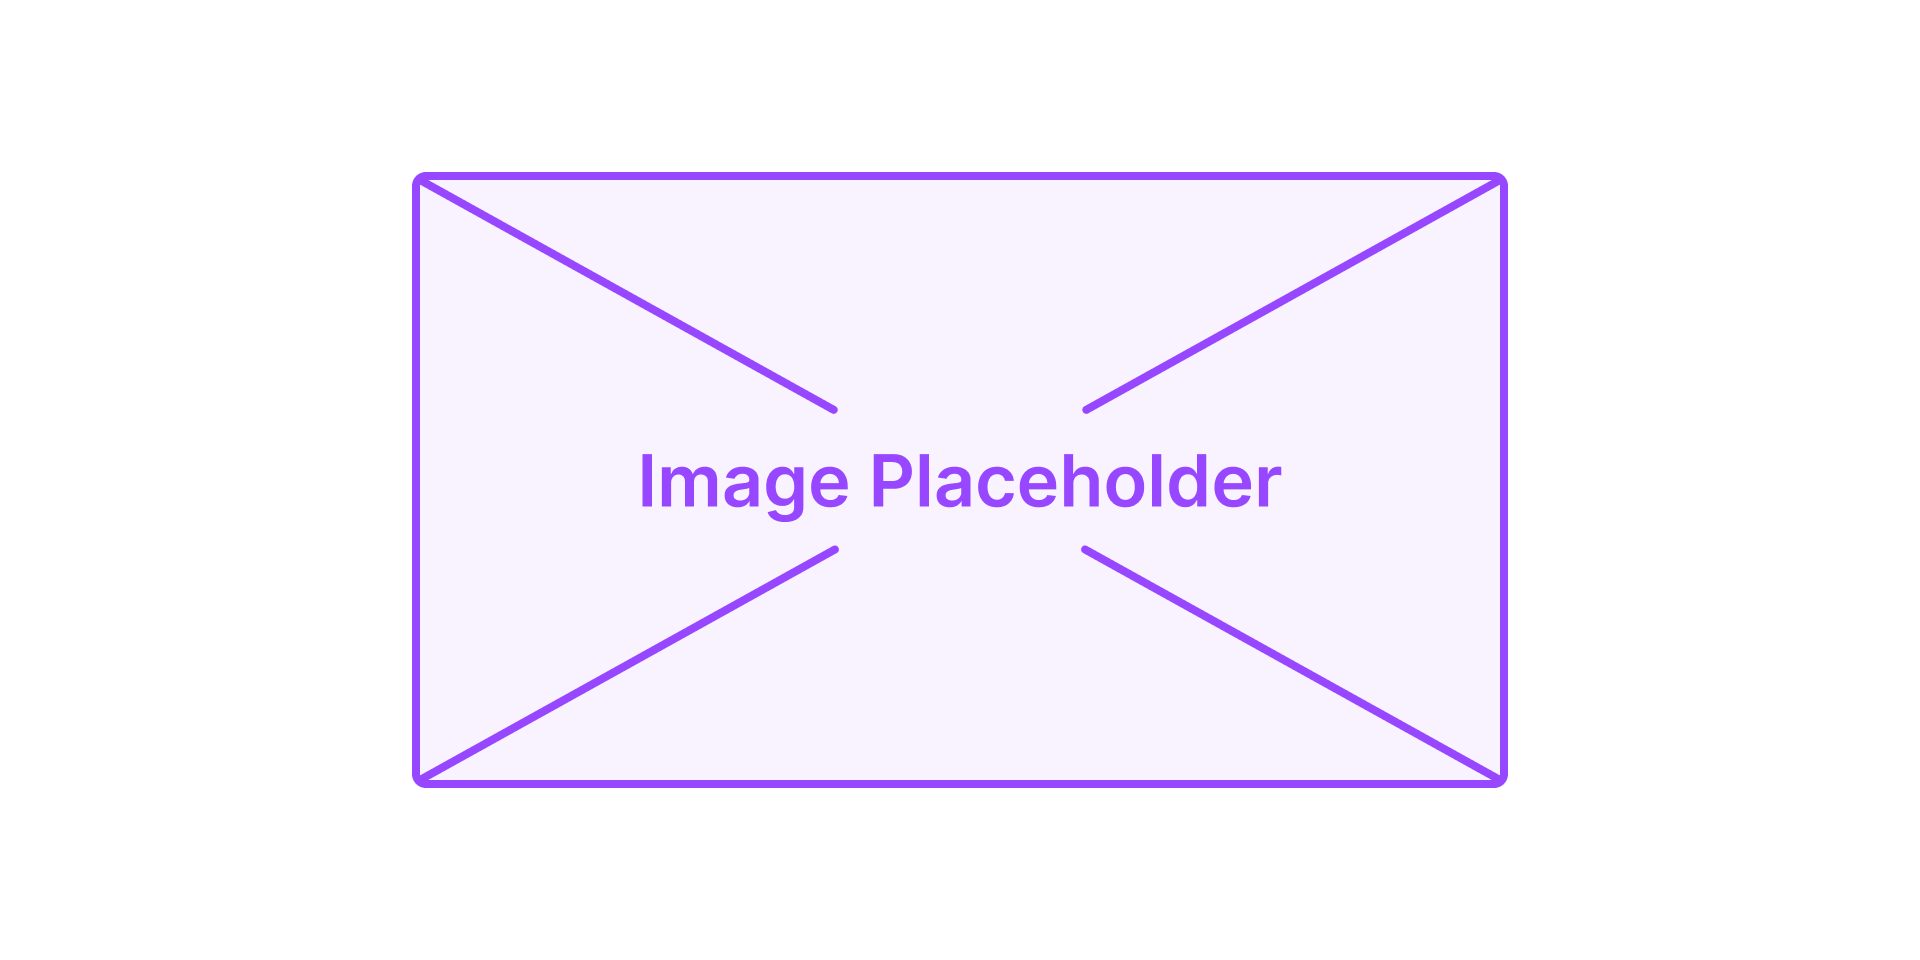
\includegraphics[width=0.9\textwidth]{graphics/placeholder.png}
    \caption{Example batch after preprocessing.}
    \label{fig:preprocessed-batch}
\end{figure}


\clearpage
\part{Methodology}
\section{Pipeline Overview}

The complete pipeline is summarized below:

\begin{center}
    \fbox{\parbox{0.96\textwidth}{\centering
    Raw data $\rightarrow$ preprocessing $\rightarrow$ data loader $\rightarrow$ model $\rightarrow$ loss\\
    $\rightarrow$ optimization $\rightarrow$ prediction $\rightarrow$ post-processing $\rightarrow$ evaluation}}
\end{center}

Replace the placeholder above with a diagram when available.
\begin{figure}[H]
    \centering
    % Suggested image filename: graphics/pipeline-overview.png
    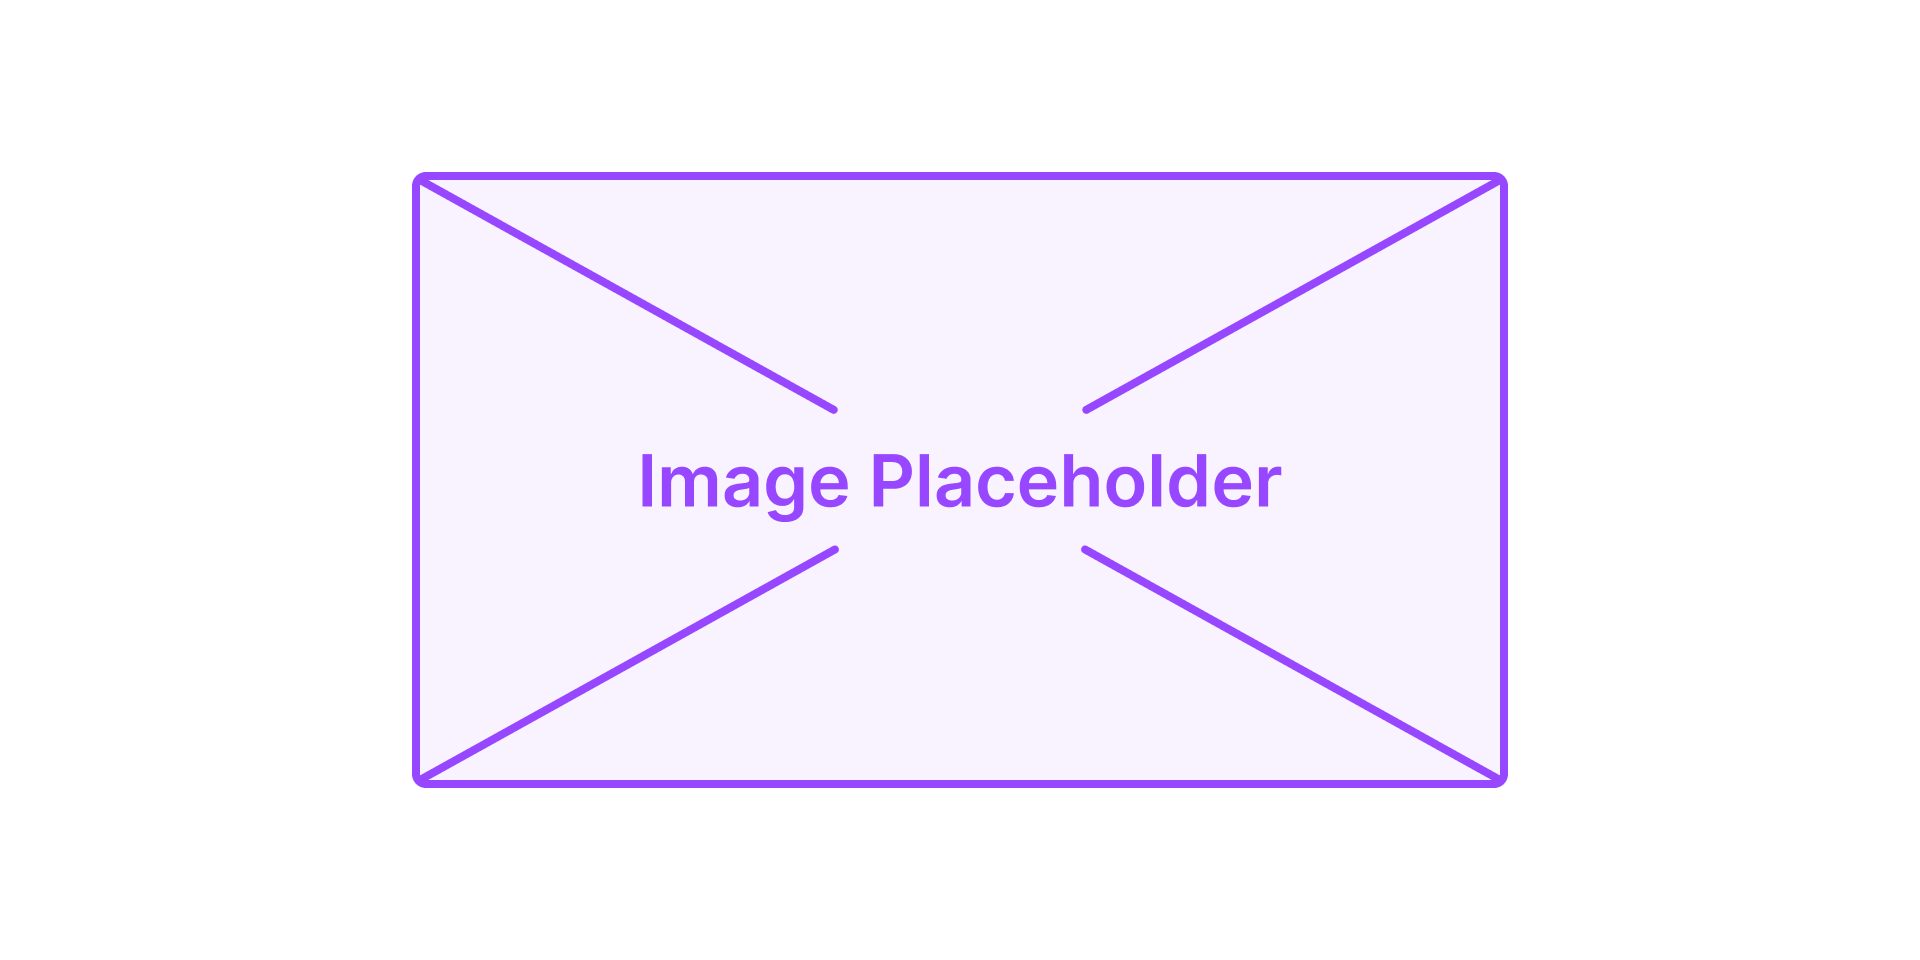
\includegraphics[width=0.9\textwidth]{graphics/placeholder.png}
    \caption{End-to-end pipeline.}
    \label{fig:pipeline-overview}
\end{figure}

\section{Baseline and Main Methods}

Describe each method's architecture, input representation, loss, metrics, strengths, limitations, and parameter count. State which components were self-implemented and which came from libraries.

\begin{table}[H]
    \centering
    \caption{Compared methods.}
    \label{tab:methods}
    \begin{tabularx}{\textwidth}{@{}lXlll@{}}
        \toprule
        Method & Architecture / input & Loss & Metrics & Parameters \\
        \midrule
        Baseline & TODO & TODO & TODO & TODO \\
        Main method & TODO & TODO & TODO & TODO \\
        \bottomrule
    \end{tabularx}
\end{table}

\section{Training Setup}

\begin{table}[H]
    \centering
    \caption{Training configuration.}
    \label{tab:training-setup}
    \begin{tabularx}{\textwidth}{@{}lX@{}}
        \toprule
        Setting & Value \\
        \midrule
        Optimizer & AdamW \\
        Learning rate & 0.001 \\
        Batch size & 256 \\
        Epochs & 10 maximum \\
        Scheduler & None \\
        Regularization & Weight decay 0.1; MLP dropout 0.2 \\
        Early stopping & Patience-style counter of 10 non-improving validation epochs \\
        Checkpoint criterion & Lowest validation loss \\
        Random seed & 42, with deterministic PyTorch algorithms enabled \\
        Hardware & TODO \\
        Mixed precision & Not used \\
        Training time & Linear: 176.43 s; MLP: 178.11 s \\
        Hyperparameter selection & Fixed configuration in `config.py`; no search results recorded \\
        \bottomrule
    \end{tabularx}
\end{table}

\section{Experimental Design}

For each experiment, state the hypothesis, changed factor, fixed factors, metrics, and conclusion criteria.

\begin{table}[H]
    \centering
    \caption{Experimental design.}
    \label{tab:experimental-design}
    \begin{tabularx}{\textwidth}{@{}lXXXX@{}}
        \toprule
        Experiment & Hypothesis & Changed factor & Fixed factors & Conclusion criteria \\
        \midrule
        EXP-01 & TODO & TODO & TODO & TODO \\
        EXP-02 & TODO & TODO & TODO & TODO \\
        \bottomrule
    \end{tabularx}
\end{table}


\clearpage
\part{Implementation Results}
\section{Training Behavior}

Learning-curve plots are generated for both models. The trainer records training and validation loss and accuracy for every epoch, then restores the checkpoint with the lowest validation loss before test evaluation. The recorded training times are 176.43 seconds for Linear and 178.11 seconds for MLP. The saved curves should be used to assess overfitting or underfitting; no separate multi-run timing analysis was performed.

\begin{figure}[H]
	\centering
	% Suggested image filename: graphics/training-curves.png
	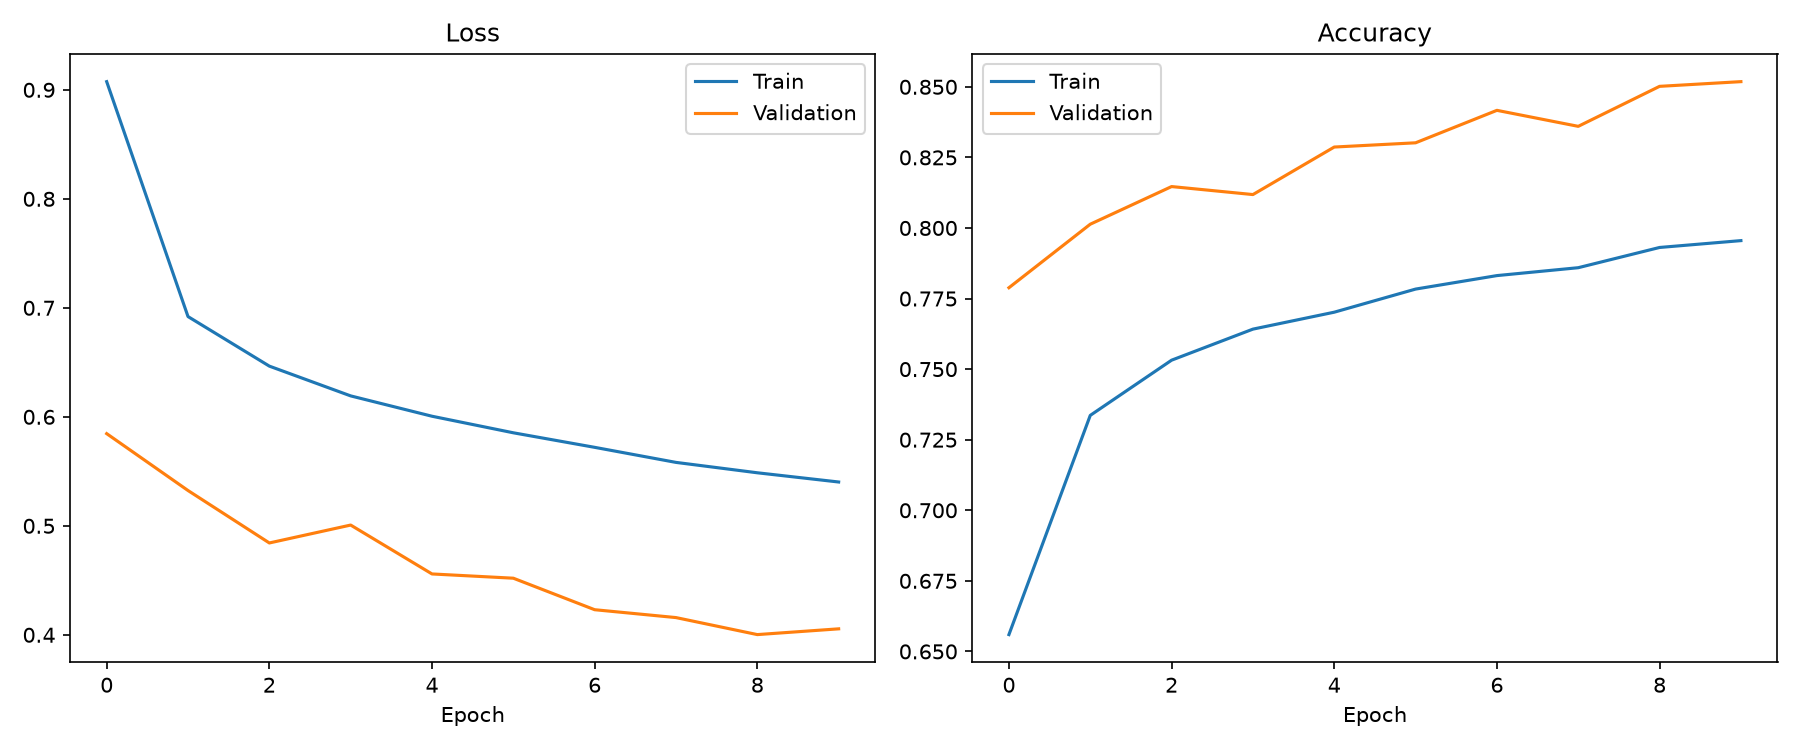
\includegraphics[width=0.9\textwidth]{../../Assignment1/outputs/learning_curves/mlp_learning_curves.png}
	\caption{MLP training and validation curves.}
	\label{fig:training-curves}
\end{figure}

The corresponding Linear learning curves are saved in 
\texttt{Assignment1/outputs/learning\_curves/linear\_learning\_curves.png}.

\section{Quantitative Results}

The following values are from the saved test metric JSON files for the single reproducible run with seed 42. Inference time is reported per sample; no multi-run mean and standard deviation were recorded.

\begin{table}[H]
    \centering
    \caption{Quantitative comparison.}
    \label{tab:quantitative-results}
    \begin{tabular}{@{}lrrrr@{}}
        \toprule
        Method & Accuracy & Macro-F1 & Parameters & Inference time \\
        \midrule
        Linear & 0.7351 & 0.7280 & 7,850 & 0.000261 ms/sample \\
        MLP & 0.8319 & 0.8269 & 567,434 & 0.004166 ms/sample \\
        \bottomrule
    \end{tabular}
\end{table}

\section{Qualitative Results}

Show correct predictions, difficult but correct cases, failures, predictions versus ground truth, and task-appropriate visualizations.

\begin{figure}[H]
	\centering
	% Suggested image filename: graphics/qualitative-results.png
	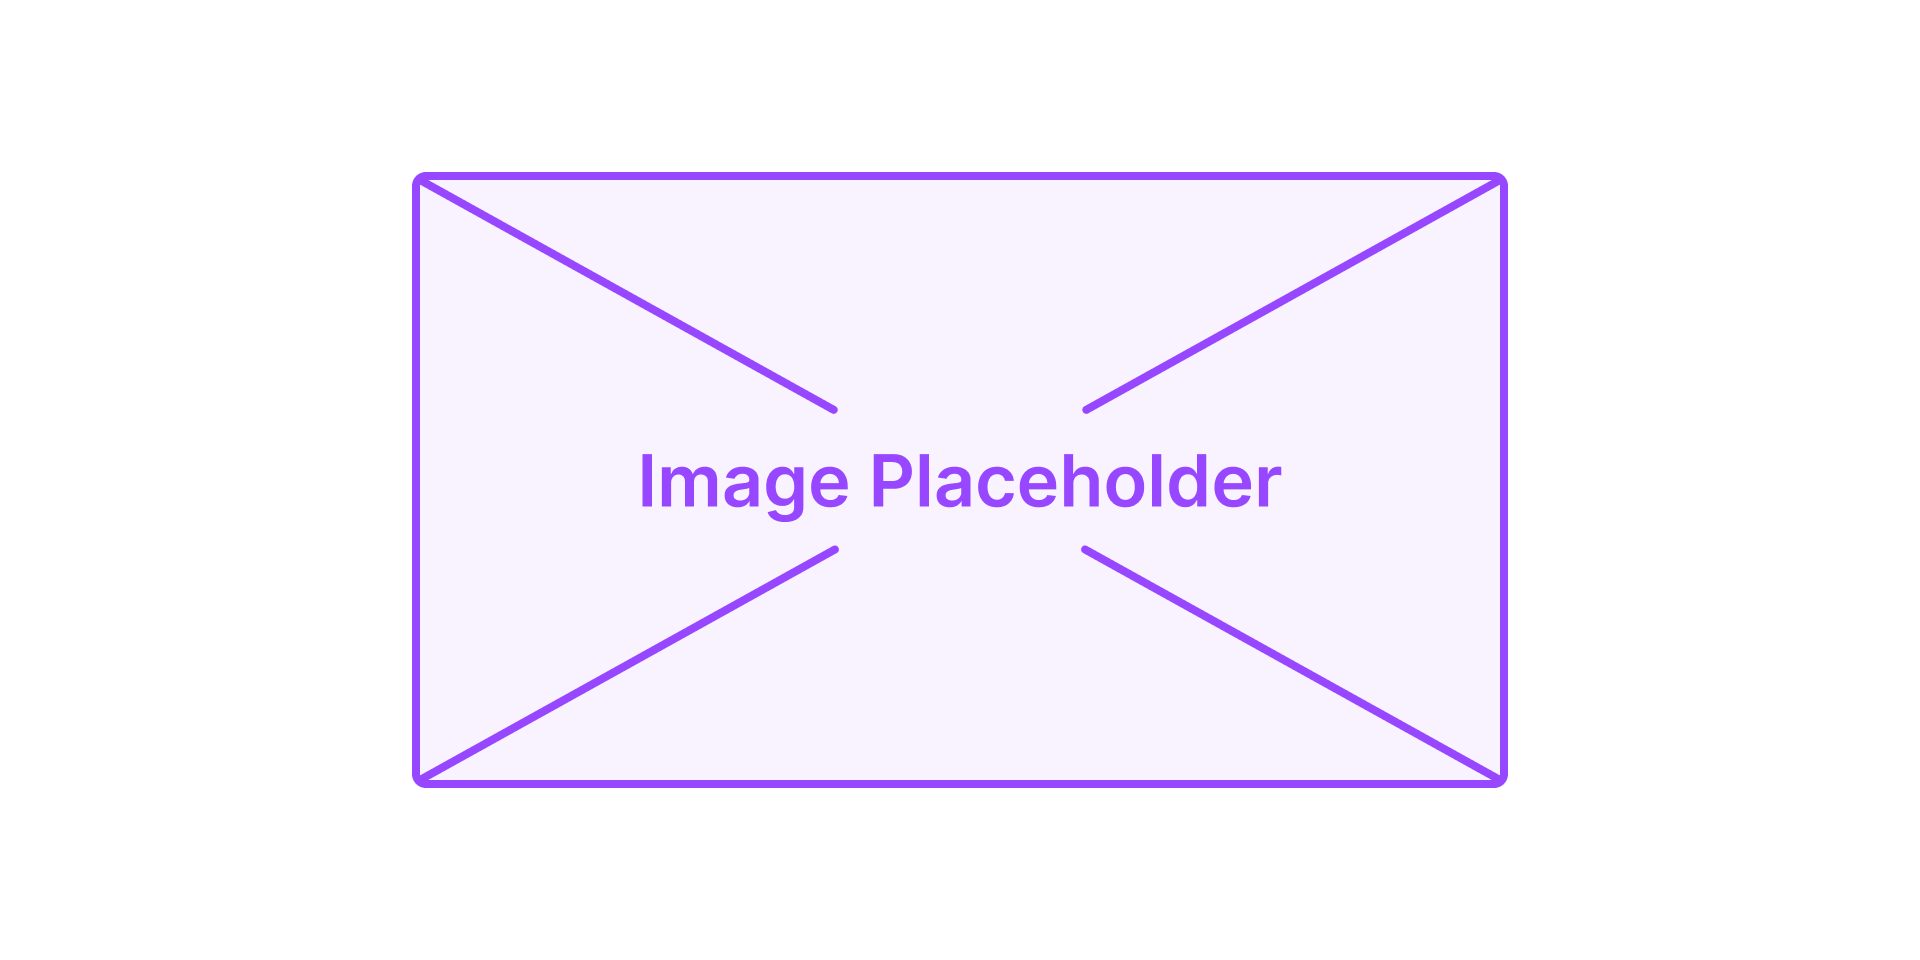
\includegraphics[width=0.9\textwidth]{graphics/placeholder.png}
	\caption{Qualitative prediction examples.}
	\label{fig:qualitative-results}
\end{figure}

\section{Comparison and Discussion}

Explain which method is better and by how much; where differences appear; causes related to data, architecture, loss, or training; accuracy--speed--parameter trade-offs; whether hypotheses are supported; and which conclusions cannot yet be drawn.

A list of metrics alone is insufficient: connect observed differences to the experimental design and evidence.

\section{Error Analysis}

For each error group, describe the error, its frequency or rate, examples, hypothesized cause, and improvement ideas.

\begin{table}[H]
    \centering
    \caption{Error groups.}
    \label{tab:error-analysis}
    \begin{tabularx}{\textwidth}{@{}lXXXX@{}}
        \toprule
        Error group & Description & Frequency / rate & Hypothesized cause & Improvement idea \\
        \midrule
        Group A & TODO & TODO & TODO & TODO \\
        Group B & TODO & TODO & TODO & TODO \\
        \bottomrule
    \end{tabularx}
\end{table}

\section{Ablation Study}

An ablation is mandatory for Assignments 2 and 3, and recommended for Assignment 1 when comparing representations or regularizers. Describe the removed or changed component and interpret the resulting performance difference.

\begin{table}[H]
    \centering
    \caption{Ablation study results.}
    \label{tab:ablation}
    \begin{tabular}{@{}lrrr@{}}
        \toprule
        Configuration & Primary metric & Secondary metric & Parameters \\
        \midrule
        Full model & TODO & TODO & TODO \\
        Without component X & TODO & TODO & TODO \\
        \bottomrule
    \end{tabular}
\end{table}

\section{Limitations and Conclusion}

Discuss data, method, and experimental limits; expected generalization; future work; and a short answer to the research question.

\textbf{Conclusion.} Summarize the evidence-based answer and avoid claims that are not supported by the experiments.


\clearpage
\section*{AI Usage Disclosure}
\addcontentsline{toc}{section}{AI Usage Disclosure}

This section records the use of generative AI tools in this assignment. All AI-assisted
content was reviewed, edited, and verified by the students. Experimental results,
performance numbers, and figures are based on actual code execution and should not be
reported solely from unverified AI output.

\subsection*{Mandatory Fields per AI Tool}

For each AI tool used, record all of the following fields:

\begin{itemize}
    \item Tool name and version or model, if known.
    \item Member who used the tool.
    \item Time or development stage.
    \item Purpose.
    \item Affected assignment section(s).
    \item Representative prompt example or prompt-log link.
    \item How the AI output was edited and verified.
    \item Member responsible for final verification.
    \item Sources used for verification, such as documentation, papers, or tests.
\end{itemize}

Suggested categories include literature search, concept explanation, architecture or
experiment design, coding assistance, debugging, test generation, report writing,
grammar checks, figure or slide generation, and result analysis.

\begin{longtable}{@{}p{0.15\textwidth}p{0.22\textwidth}p{0.25\textwidth}p{0.28\textwidth}@{}}
    \caption{AI usage disclosure log.}
    \label{tab:ai-usage-log}\\
    \toprule
    Field & Entry 1 & Entry 2 & Entry 3 \\
    \midrule
    Tool and version/model & TODO & TODO & TODO \\
    Used by & TODO & TODO & TODO \\
    Time / development stage & TODO & TODO & TODO \\
    Purpose & TODO & TODO & TODO \\
    Affected sections & TODO & TODO & TODO \\
    Prompt example or log link & TODO & TODO & TODO \\
    Editing and verification & TODO & TODO & TODO \\
    Responsible member & TODO & TODO & TODO \\
    Verification sources & TODO & TODO & TODO \\
    \bottomrule
\end{longtable}

\subsection*{Disclosure Example}

\begin{description}
    \item[Tool:] [Tool/model name]
    \item[Used by:] [Member name]
    \item[Development stage:] [Time or stage]
    \item[Task:] Debugging the validation loop in \texttt{train.py}
    \item[Prompt summary:] Asked why validation loss was accumulated incorrectly.
    \item[AI contribution:] Suggested sample-weighted loss accumulation.
    \item[Student verification:] Compared the suggestion with PyTorch documentation and tested it on a small controlled set.
    \item[Affected files/sections:] \texttt{src/train.py}; Report Sec.~3.2.
    \item[Responsible member:] [Member name]
    \item[Sources used for verification:] [Documentation, papers, or tests]
\end{description}





% \section*{GitHub Repositories}
% \addcontentsline{toc}{section}{GitHub Repositories}

\printbibliography

\nocite{*}

\end{document}